% Experiments: hand-written transformers. Owner: claude-13.
\subsection{Transformers with hand-written attention}
\label{sec:transformer}

The networks so far are convolutional, recurrent or feed-forward. A reader may
grant that heuristics can be packed into those and still doubt that
\emph{attention}---the operation that defines current models---can be written by
hand. This section writes three transformers whose correctness is exact, on tasks
chosen because mechanistic interpretability has reverse-engineered the same
circuits out of trained models \cite{olah2020zoom}. We build them forward.

\paragraph{Architecture.} A decoder-only transformer in numpy: token and position
embeddings, $L$ layers of causal multi-head attention and a ReLU MLP with residual
connections, and an unembedding. There is no LayerNorm: every dimension of the
residual stream is given a name by the author (\texttt{s}, \texttt{nine},
\texttt{carry}, \texttt{prev[7]}, \dots) and a fixed scale, which normalisation
would destroy. All tensors are allocated at full shape and zero; \texttt{to\_torch()}
yields the identical module, and with random initialisation, its trained twin.

\paragraph{Addition with carry.} The input is the two addends as digit pairs,
least-significant first, after a BOS token and with one extra $0{+}0$ column for the
final carry; the output at column $i$ is digit $i$ of the sum. The embedding of a
pair $(a,b)$ is the column sum $s=a+b$ together with the flags $[s=9]$ and
$[s\ge10]$. The only hard part of addition is the carry chain: the carry into
column $i$ is decided by the nearest earlier column whose sum is not nine, since
nines pass a carry through unchanged. One attention head finds that column:
$\mathrm{score}(i,k) = 200\,(1-\mathrm{nine}_k) + 5\,\mathrm{pos}_k$ under a strict
causal mask, so ``not nine'' dominates, recency breaks ties, and softmax gaps of at
least 5 make the pattern close to one-hot (0.993 on $999999+1$,
Figure~\ref{fig:attn}). Its value is that column's $[s\ge10]$, written into a
\texttt{carry} dimension; BOS acts as a decider with carry~0. The MLP then
computes $(s+\mathrm{carry}) \bmod 10$ with 21 units $\mathrm{relu}(s+\mathrm{carry}-j)$,
$j=-1,\dots,19$, whose differences $\mathrm{relu}(x-k+1)-2\,\mathrm{relu}(x-k)+\mathrm{relu}(x-k-1)$
are triangular bumps equal to 1 at $x=k$ and 0 at every other integer; bump $k$
adds one to output digit $k \bmod 10$. One layer, one head, 2{,}851 parameters, 405
non-zero; exact on 2{,}000 random problems of up to twelve digits.

\paragraph{Dyck-1.} Is a bracket string balanced? Opening and closing brackets
embed as $\pm1$. A layer-1 head with all scores zero attends uniformly over
positions $0..i$ and so outputs $\mathrm{depth}_i/(i+1)$; its MLP produces
$\mathrm{neg}_i=\min(\mathrm{relu}(-C\,\mathrm{depth}_i),1)$ with $C$ above the
maximum length, so any negative prefix registers as exactly 1, and likewise a
non-zero flag. A layer-2 head with $\mathrm{score}(i,k)=30\,\mathrm{neg}_k$
concentrates on any flagged position and reads 1, or stays uniform over unflagged
positions and reads 0: ``was any prefix negative?'' The string is invalid if that
or the final non-zero flag fires. Two layers, 654 parameters, 26 non-zero; exact
on 2{,}000 strings of up to 48 brackets, half balanced and half near-misses.

\paragraph{Induction.} Given $x_1..x_L\,x_1..x_k$, predict $x_{k+1}$. A layer-1
``previous token'' head ($\mathrm{score}=8\,\mathrm{pos}_k$, strict causal mask, so
$i-1$ wins) copies the previous token's one-hot into a \texttt{prev} block. A
layer-2 ``induction'' head uses the current token as query and \texttt{prev} as key
(score 20 on a match, plus $0.5\,\mathrm{pos}_k$ so the most recent match wins when
a letter repeats) and returns that position's token: what followed last time. Two
layers, 25{,}336 parameters, 278 non-zero; exact on patterns of distinct letters.

\begin{figure}[t]\centering
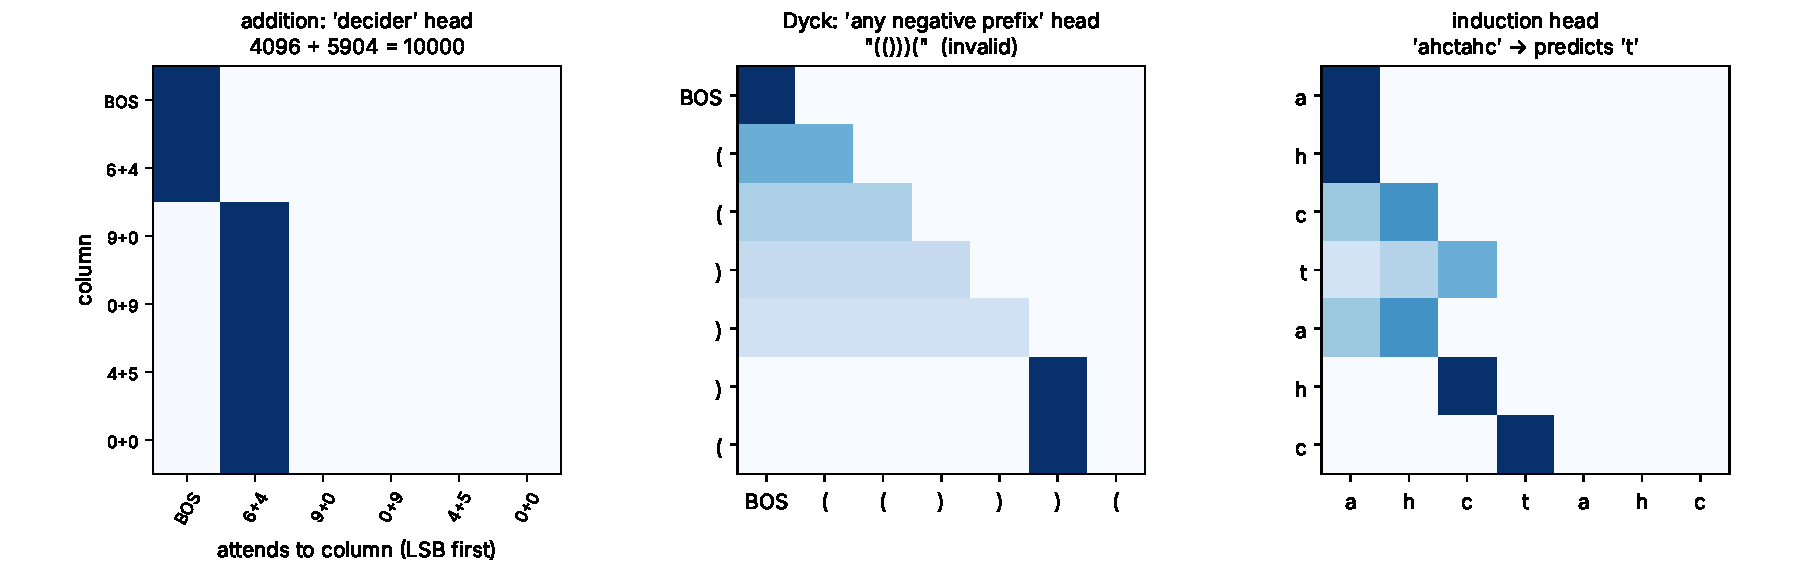
\includegraphics[width=\linewidth]{figures/transformer_attention.pdf}
\caption{Attention patterns of the hand-written heads. Left: in $4096+5904$ every
column after $6{+}4$ attends to it, because the intervening columns all sum to nine
and the carry chain runs through them. Middle: the Dyck head locks onto the bracket
at which depth first went negative. Right: the induction head attends from each
letter of the second copy to the successor of its first occurrence.}
\label{fig:attn}
\end{figure}

\paragraph{Trained twins.} Table~\ref{tab:transformer} trains the identical
architecture from random initialisation on $2^k$ examples (Adam, 3{,}000 steps) and
reports the same exact-match metric. The designed networks are exact with no
labels. The trained twins are near chance at 64--256 examples, reach 97--99\,\%
at $2^{10}$, and at $2^{14}$ are still not exact (95--99.7\,\%; the addition
twin's dip at $2^{14}$ is training variance under a fixed step budget). The gap
between 99.7\,\% and 100\,\% is the gap between a statistical approximation of the
carry rule and the rule itself.
\begin{table}[h]\centering
\begin{tabular}{lcccccc}\toprule
labels seen & 0 (designed) & $2^{6}$ & $2^{8}$ & $2^{10}$ & $2^{12}$ & $2^{14}$ \\\midrule
addition & 100.0 & 7.7 & 25.9 & 97.4 & 99.0 & 95.2 \\
dyck & 100.0 & 64.4 & 68.0 & 98.3 & 98.7 & 98.7 \\
induction & 100.0 & 5.6 & 37.2 & 98.6 & 99.6 & 99.7 \\
\bottomrule\end{tabular}
\caption{Exact-match accuracy (\%) of the hand-written transformers (0 labels) and of the same architecture trained from random initialisation on $2^k$ examples, 3{,}000 Adam steps, 1{,}000 held-out problems. Addition: whole sum correct; Dyck: validity; induction: next token in the second copy.}
\label{tab:transformer}
\end{table}

